\chapter{Results}\label{chap:results}
\section{Convergence Test}
\begin{table}[htb]
  \centering
\caption{Numerical order of convergence of ADER-DG method}%
\label{tab:convergence-order}
\begin{tabular}{@{}lS[table-format=1.2]S[table-format=1.2]S[table-format=1.2]@{}}
\toprule
{Order} & {$L_1$} & {$L_2$} & {$L_\infty$}\\ \midrule
1 & 2.03 & 2.00 & 1.92\\
2 & 2.56 & 2.55 & 2.55\\
3 & 3.43 & 3.40 & 3.44\\
4 & 4.44 & 4.44 & 4.67\\
5 & 5.37 & 5.34 & 5.28\\
6 & 5.43 & 5.42 & 5.30\\
\bottomrule
\end{tabular}
\end{table}

\begin{figure}[htb]
  \centering
  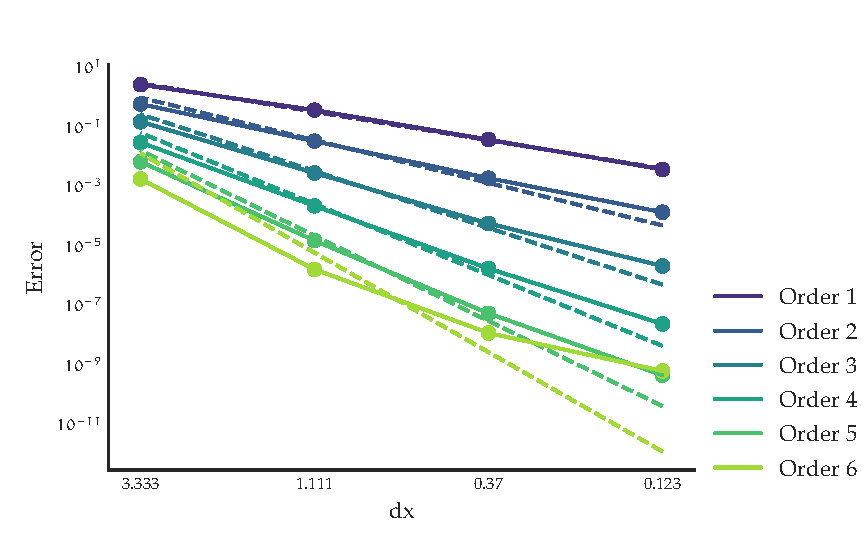
\includegraphics{thesis_convergence}
  \caption{$L_2$-Error vs.\ Grid Size}
  \label{fig:convergence-l2-error}
\end{figure}

\newcommand{\error}{\operatorname{Total-Error}}

Before computing the error we first need to define the $L_p$ norms for a $p > 0$ by
% notation: https://en.wikipedia.org/wiki/Lp_space#Lp_spaces
\begin{equation}
  \label{eq:Lp-nrom}
  \Vert f(x) \Vert_p = \left( \int_K \vert f(x) \vert^p d\mu  \right)^{1/p}.
\end{equation}
We are interested in the total error which we define as the norm of the difference between an analytical solution $f(\bm{x}, t)$ and our approximation $\hat{f}(\bm{x}, t)$.
The error at a time $t$ is thus defined as
\begin{equation}
  \label{eq:error}
  \error(t,p) = \Vert f(\bm{x}, t) - \hat{f}(\bm{x}, t) \Vert_p.
\end{equation}

We first observe that for our approximation space $\broken$ we can split up the error as a sum over all cells
\begin{equation}
  \label{eq:lp-norm-broken}
 %\Vert f(\bm{x}) \Vert = \sum_{\cell[] \in \broken} \Vert f_{\cell[]} (\bm{x}) \Vert_p,
  \error(t,p) = \sum_{\cell[] \in \broken} \error_{\cell[]}(t,p)
\end{equation}
where $\error_{\cell[]}$ is the error in the cell $\cell[]$.

\todo{Describe how to integrate the error for cells, and effect of volume}
We evaluate the cell-wise error with Gaussian quadrature using \cref{eq:integration-by-substitution}
 \begin{equation}
   \Vert f_K(x) \Vert_p = \left( V \sum_{\bm{i}} \vert f(\bm{x}_i, t) - \hat{f}(\bm{x}_i, t) \vert^p w_{{\bm{i}}}  \right)^{1/p},
 \end{equation}
where $V = \Delta x \Delta y$ is the volume of each two-dimensional cell.
The sum runs over all quadrature nodes $x_i$ with weights $w_i$.
We use ten nodes.

For the limiting case of $p \to \infty$ we use the maximum point-wise error.


We compute the error for the manufactured-solution scenario (\cref{sec:manufactured-solution}).
Looking at the plot for the $L_2$ error (refer to plot here) shows that our method converges for all tested polynomial orders.
\todo{Preliminary results used here!}

To compute the numerical order of convergence, we perform a linear regression of the logarithm of the error vs.\ the logarithm of the meshsize.
The size of the slope is then the convergence order.
We can see (\cref{tab:convergence-order}) that our numerical convergence rate increases with the polynomial order.
We do not achieve the optimal theoretical order of convergence of $N+1$.
In~\cite{dumbser2010arbitrary}, which use a similar numerical method and the same scenario, but a different grid, \citeauthor{dumbser2010arbitrary} achieves the optimal order for most polynomial orders.
Some \textsc{dg}-methods of odd order only achieve a numerical convergence order of $N+\nicefrac{1}{2}$.

\section{Accurate CFD}
\section{Accurate Clouds}
\section{AMR Efficiency}
To show the effectiveness of the \amr{}, we compare the time to solution of a simulation using \amr{} and another simulation with a fully refined mesh.
In detail, we compare
\begin{description}
\item[AMR] We use a coarse mesh with just $9 \times 9$ cells.
  Each cell can be refined up to three times.
  That is, the cells have sidelengths of roughly $\left( \SI{111.1}{\m}, \SI{37.04}{\m}, \SI{12.35}{\m} \right)$.
  As refinement thresholds we use $T_\text{refine} = 2.5$ and $T_\text{delete} = -0.5$ in \cref{eq:refinement-criterion}.
\item[Fine] We use a uniform grid where all cells have a sidelength corresponding to the finest mesh of the \amr{}-test case.
  In addition, we disable the reduction of global observables.
\end{description}
We use an \aderdg{}-method of order $4$ and thus have a minimal effective resolution of ca.\ $\SI{3.09}{\m}$.

To ensure a fair comparison, we ran both configurations with the same optimisation option.

We use a single node of the Haswell-nodes of the Supermuc (Phase 2).
The node has two xxx \textsc{cpu}s with 28 cores each.
We use the \tbb{} parallelisation of \exahype{}.
To find a reasonable parameter for the number of background threads, we ran a grid search.
We ran three \arm{} testcases for a simulation time of $\SI{1}{\min}$.
The best median performance was achieved by only using two background threads!

\section{Reactive Euler \textit{\&} Navier Stokes}

%%% Local Variables:
%%% mode: latex
%%% TeX-master: "../main"
%%% End:
